
\documentclass[letterpaper]{article}
\usepackage{lscape}
\usepackage{comment}
\usepackage{geometry}
\usepackage{graphicx}
%\usepackage{palatcm}

\geometry{left=1in,right=1in, top=1in, bottom=1in}



\begin{document}

%\qcjtitle{\sc{(SUPPLEMENTARY)}}{\sc{A Model for Sequencing Bias in RNA-Seq}}{Daniel C. Jones}

%\begin{center}
%\large{
%\sc{SUPPLEMENTARY}

%\sc{A model for Sequence Bias in RNA-Seq}
%}
%\end{center}


\section{Trimming Reads}

Observing the nonuniform distribution of nucleotide frequencies surrounding the
5' end reads, a natural step to take would be to trim the 5' end before mapping,
in the hope that simply removing the portion of the read in which the bias
occurs will also remove the bias. The figure below demonstrates that this is not
the case. Trimming the initial heptamer in the Mortazavi data set does nothing to
reduce the bias, and simply shifts the plot by seven positions. This indicates
that the issue is \emph{sampling bias}, rather than a bias in base calling.


%% TODO
\begin{comment}
%\begin{figure}[b]
\begin{center}
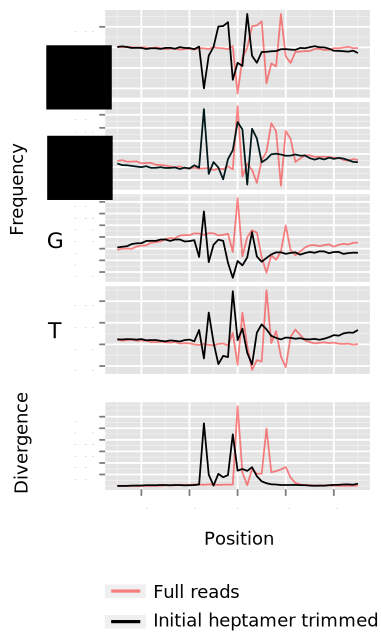
\includegraphics[width=0.35\textwidth]{fig/trimmed-freqs.pdf}
\end{center}
%\caption{Nucleotide frequencies for trimmed and untrimmed reads from the
%Mortazavi dataset.}
%\label{fig:trimmed}
%\end{figure}
\end{comment}


\section{CHiP-Seq}

Though we found the MART model \cite{Li2010} to be competitive with our own,
yet ours offers the advantage that no gene annotations are needed for training. In
RNA-Seq this is useful in applications of de-novo gene discovery, but it also
allows our method to be applied to CHiP-Seq and another short read data. Here we
examine one publicly available CHiP-Seq data set from Cao, et. al.
\cite{Cao2010}.  

Measuring nucleotide frequencies, we find the bias to be significantly less
than that observed the RNA-Seq data sets we tested, but the data was by no means
unbiased.

%% TODO
\begin{comment}
%\begin{figure}[b]
\begin{center}
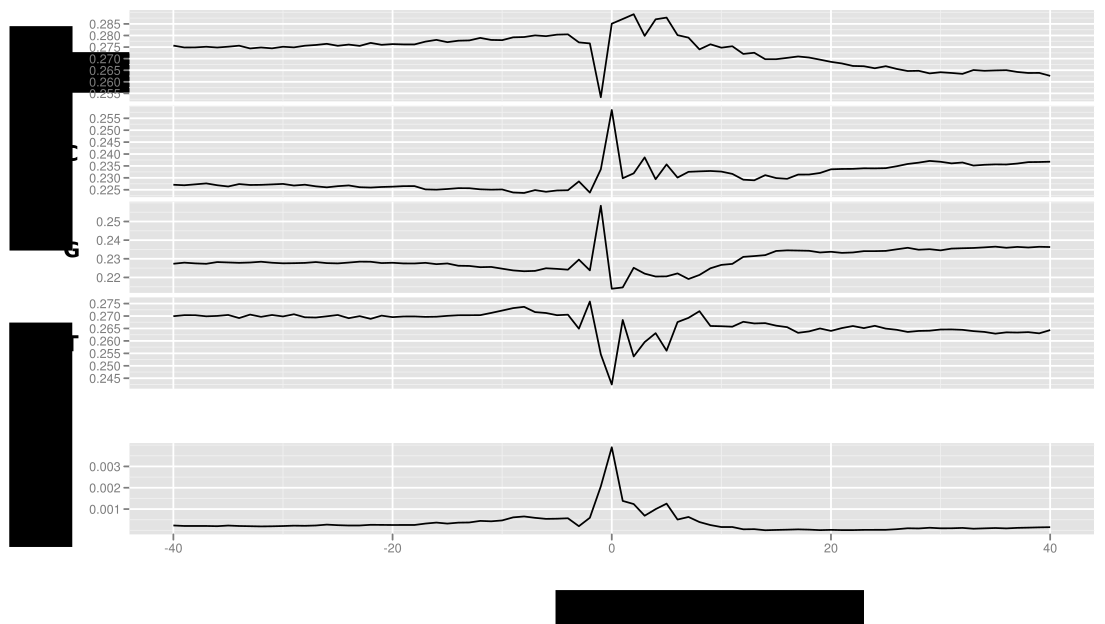
\includegraphics[width=0.5\textwidth]{fig/freqs_cao.pdf}
\end{center}
%\caption{Nucleotide frequencies from CHiP-Seq reads.}
%\label{fig:freqs_cao}
%\end{figure}
\end{comment}

In the analysis of the RNA-Seq data, we used the assumption of continuous
transcription across annotated exons to evaluate the efficacy of the models, as
well as to train the GLM and MART models. Evaluating bias correction on CHiP-Seq
data necessitates dropping the Poisson regression test, as well as the GLM and
MART models from our comparison, which can not be applied to such data.

We did however repeat our analysis using the Kullback-Leibler divergence.  We
trained each method using reads from reads from chromosomes 1--8. The remaining
chromosomes were segmented into 500nt bins, and the KL divergence was sampled
from the 50,000 segments with the highest read counts.

First we plot directly the positional KL divergence, computed identically 

%% TODO
\begin{comment}
\begin{center}
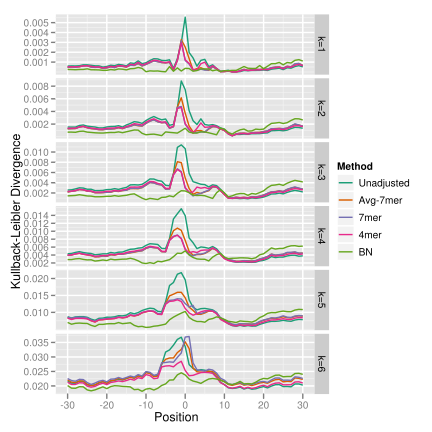
\includegraphics[width=0.5\textwidth]{fig/cao-kl.pdf}
\end{center}
\end{comment}

Secondly, we summarize these plots, computing one normalized divergence
estimate by summing the KL divergence of positions -20 through 20, and
divided by the unadjusted summed divergence to normalize.

%% TODO
\begin{comment}
\begin{center}
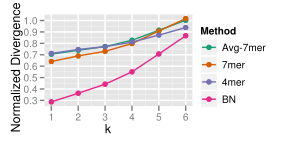
\includegraphics[width=0.5\textwidth]{fig/cao-kl-delta.pdf}
\end{center}
\end{comment}

We see that our method is effective at reducing the bias in this ChiP-Seq data.


\section{Variability Between Replicates}

Measuring differential expression or isoform switching is a primary application of
RNA-Seq. If the bias were inconsistent between replicates, it would call into
question the accuracy of such tests. In our experiments, we have observed the
bias to be mostly, but not entirely consistent between replicates. Below, we
plot the frequencies from the four runs in the Trapnell data set.

%% TODO
\begin{comment}
\begin{center}
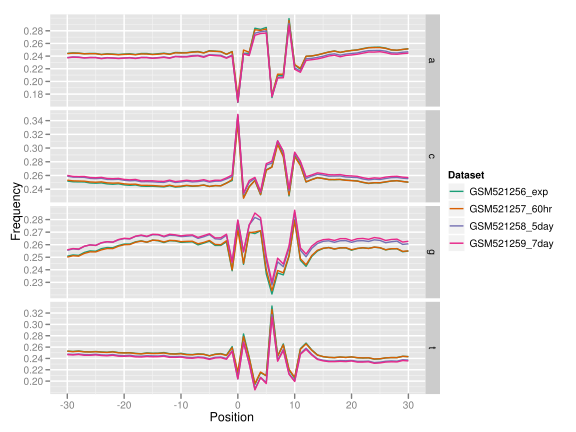
\includegraphics[width=0.5\textwidth]{fig/replicates.pdf}
\end{center}
\end{comment}

Though we do not know if the variability is always minor, assuming this is so,
there remains the risk that the sequence bias would greatly effect the depth to
which a locus is sequenced, and thus the statistical significance of
differential expression tests. This would bias the discovery of differentially
expressed genes, but not the test itself.



\section{Additional Plots}

Below we plot the adjusted and unadjusted KL divergence of each sample.

%% TODO
\begin{comment}
%\begin{figure}[b]
%\begin{center}
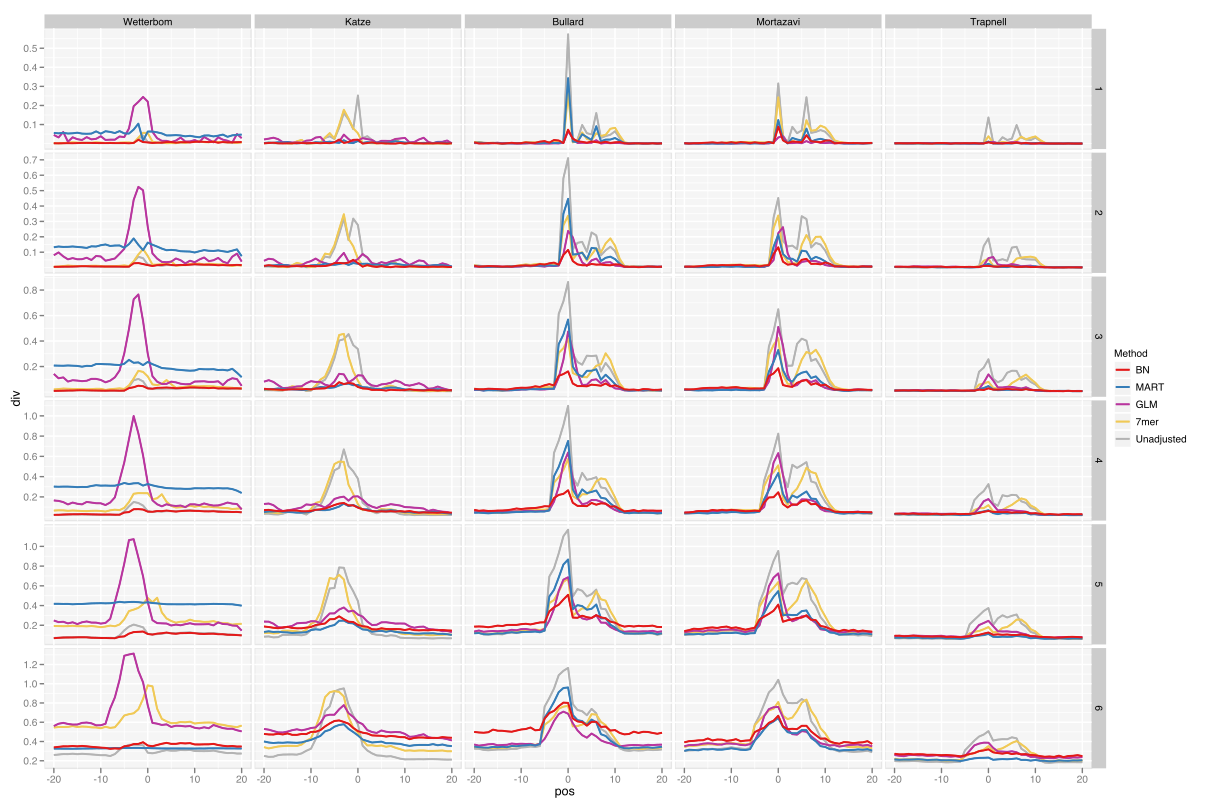
\includegraphics[width=\textwidth]{fig/kl-all.pdf}
%\end{center}
%\caption{Positional KL divergence for each dataset and method.}
%\label{fig:kl-all}
%\end{figure}
\end{comment}


\bibliographystyle{plain}
\bibliography{seqbias-supplement}

\end{document}

